\chapter{The  Heart}

\section{introduction to the heart and its functions}
%%\label{sec:multicore_architectures}
%%Maybe quotes instead?
The heart. The most iconic organ in the human body, responsible for thousands of bad love songs and poorly made decisions. While in reality, the heart is actually a big muscular pump that powers the entire circulatory system, transporting mainly oxygen, nutrients, hormones and heat throughout the body. 

\section{Layers of the Heart Wall}
The heart consists of three layers, the \textit{epicardium}, \textit{myocardium}, and the \textit{endocardium}. 

The outermost layer is called the epicardium. The epicardium is a thin layer of connective tissue [19], and fat that serves as a protection from trauma as well as lubricant for the sorrounding environment. 

The heart is constructed with a special kind of muscle tissue called the myocardium, also referred to as the cardiac muscle. Which makes up the majority of the thickness and mass of the heart. The cardiac muscle is one of the main reasons to why the heart pumps blood. When the cardiac muscle cells receives electrictrial stimulation, it results in a rhytmic contraction and relaxtion phase, that makes the heart beat. A deeper description of the electrophysiological process in the heart can be found in section [X.X]

The endocardium is the innermost layer in the heart wall. bla bla

%%which is one of four tissues that supports, connects or separates different types of organs and tissues in the body [19] FOOTNOTE?

\section{Composition of the Heart}
To get an illustrative perspective of the composition of the heart, it helps think of it as a student apartment that is made up of a left and right unit. The left and right unit are seperated by a wall known as a cardiac septum. Student housings are known to be space saving, so each unit is then subdivided into a upper chamber referred to as the \textit{atrium}, and a lower chamber known as the \textit{ventricle}, as illustrated in [FIGURE X.X]. The right atrium (RA) is above the right ventricle (RV), while the left atrium (LA) sits above the left ventricle (LV). The atria is responsible for receiving blood, meaning that the RA and LA are connected to veins which carry blood to the heart. The RA receives blood from the vein called the vena cava, while the LA receives blood from the four pulmonary veins which stems from the lungs. The ventricles are responsible for pushing blood away from the heart. The RV pushes blood through the pulmonary artery, and into the lungs, while the LV is responsible for pushing the blood into the \textit{aorta}, and throughout the entire body.

\begin{figure}[h]
 \centering 
     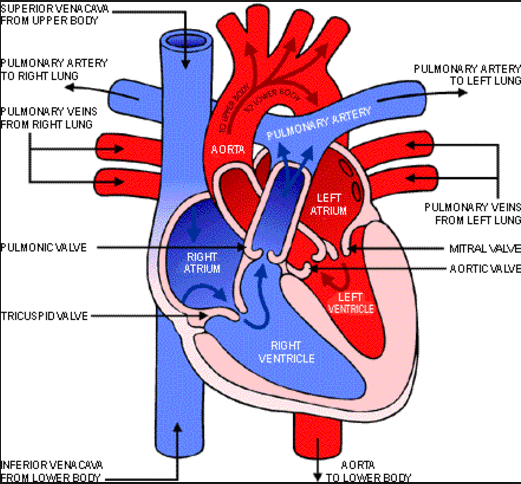
\includegraphics[width=0.9\textwidth]{bilder/b_heart_structure_new}
     \caption{Explaining the decomposition process in a 3 dimensional structured mesh. Illustration taken from \cite{article9}.
     \label{b_heart_structure_new.png}}
\end{figure}

If we were to take our student apartment example even further, the only way of getting into or leaving the lower chambers is by passing the valves. The valves are made of connective tissue \cite{article17}[FOOTNOTE] that acts like flaps. It helps think of the valves as one-way entranced doors that only has two states, open and closed. When the chambers are filled up with blood, and the pressure is greater behind the valve, the cusps (also referred to as leaflets) opens  \cite{article22}. Similarly, when the pressure is greater in front of the valve, the cusps closes, preventing any blood from flowing backwards. 

The valves can be divided into two types, \textit{semilunar} and \textit{atrioventricular} valves \cite{article19}. \textit{The atrioventricular valve} (AV) separates the atria from the ventricles. The atrioventricular valves are attached to tough strings called \textit{chordae tendinea} that connects the edges of the \textit{tricuspid} and  \textit{mitral valve} to papillary muscles. When the papillary muscles contract, it effectively prevents the AV from flopping backwards. \cite{article18}

The  AV that separates the RA and RV is the triscupid valve, due to its three cusps. The AV on the left side of the heart is the mitral valve, also called the bicuspid valve, due to its two cusps. 

The semilunar valves (SV) does not have a chordae tendinea to prevent them from overextending \cite{article20}, instead the leaflets are shaped like a cup to prevent blood from flowing backwards, and use the blood pressure to close its cusps. The Pulmonic valve is located on the left right side of the heart, while the aortic valve is located on the left side.

\begin{figure}[h]
 \centering 
     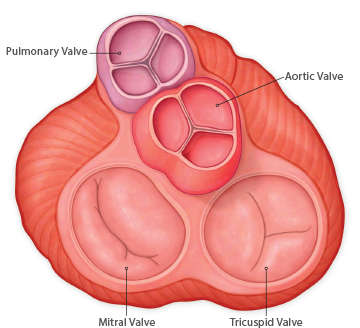
\includegraphics[width=0.9\textwidth]{bilder/b_heart_valves}
     \caption{\cite{pic4}}.
     \label{b_heart_valves.png}
\end{figure}


The right side of the heart consists of a thinner myocardium compared to the left side. The difference in size is related to its functions. The right side of the heart ensures a pulmonary circulation by sending blood to the lungs. The left side of the heart sends blood through the aortic vessel and all the way to the extremeties of the body. Since blood that originates from the left side travels a greater distance compared to the right side, it needs to be sent away with greater force, and thus have a thicker myocardium.

%%If we were to take our student apartment example even further, the only entrance for getting into the left unit is located in the right atrium. This is a one-way entrance, meaning that students can only enter 
%%[http://www.hopkinsmedicine.org/healthlibrary/conditions/
%%cardiovascular_diseases/anatomy_and_function_of_the_heart_valves_90,
%%P03059/]
%%bilde her!


%%the primary function of the cardiovascular system is to supply body cells with nutrient material and carry away waste products
%%, and it does not care about poetry or emotions.

\section{The Blood Flow in the Caridovascular System}
An understanding of the circulation of blood through the heart might help the reader to get an better understanding of how the different parts of the heart relate. It helps think of all the blood vessels in the body as a huge sophisticated railway network, where essentially alle the blood in the veins throughout the body ends up in the vena cava, the railway end station. The superior vena cava receives blood from the upper part of the body, whereas the inferior vena cava receives blood form the lower part of the body. As the blood fills up in the RA, the increasingly pressure eventually makes the tricuspid valve shut open, allowing deoxygenated blood [FOOTNOTE] to enter the RV. As the deoxygenated blood flows into the RV, the pressure in front of the tricuspid valve eventually exceeds the pressure behind the valve, resulting in the tricuspid valve to close the cusps. 

As later described in section [X.X] the cardiac cycle includes a contraction followed by a relaxation phase [HEART BOOK]. When the RV contracts, the pulmonic valve opens, allowing deoxygenated blood to enter the pulmonary artery and into the right and left side of the lungs. In the lungs, the carbon dioxide that was added to the red blood cells throughout the body is exhanged for a fresh supply of oxygen \cite{article21}.
As the LA gets filled with oxygenated blood, the mitral valve will eventually respond to the increasingly pressure behind the valve by allowing blood to enter the LV in the same way as the tricuspid valve. When the LV contracts, the aortic valve opens and the oxygenated blood gets pushed into the artery called the aorta. From the aorta, the freshly oxygenated blood gets sent throughout the body.

By now, the reader should have a basic understanding of how the heart works. Yet one important question remains unanswered, what makes your heart beat?

\section{The Electrical Activity in the Cells}
The pumping function of the heart relies on a collective, rhytmic cycle of contraction and relaxation of billions of muscle cells, more specifically, about \(10^{10}\) muscle cells [HEART BOOK]. One of the main reason to why the heart is able to contract and relax is due to the fact that the cardiac cells are excitable, meaning that the cells are able to respond actively to electric stimulus [HEART BOOK]. During the resting phase, the cells are abel to maintain an internal ionic concentration different than those of their surroundings. A cell membrane acts a barrier that sepparates the interior of the cells from the outside environment. A potential difference arises across the cell membrane due to electrically charged ions. The potential difference are referred to as the \textit{transmembrane potential}. The transmembrane potential typically varies from \(-70\) to \(-100\) mV [HEART BOOK] when there is no electric stimulus, also referred to as the resting phase. 

If an eletric stimulus is applied to the muscle cells it results in a change in the potential difference. The cells may react to an potential change, caused by an electric stimulus in one of two ways. If the applied electrical current is too small, the conductive properties of the cell will remain membrane unchanged. When the applied electric stimulus stops, the transmembrane potential quickly returns to its resting state, more specifically, the cells remains its internal negative ionic concentration [HEART BOOK]. If the electrical current is strong enough for the transmembrane potential to reach a certain threshold. It will cause a rappid flux of positive ions into the cell [HEART BOOK]. This phase is referred to as a \textit{depolarization} phase. A depolarization of the membrane causes the transmembrane potential to increase from its negative resting state, to a value around \(0\) mV, or significantly above, depending on the ionic current. The transmembrane potential will gradually return back to its negative resting state, a process referred to as a repolarization of the membrane. The complete process in which a depolarization and repolarization ouccurs, is called an action potential. 

\section{Signal Conduction}
The process of electrical signals that propagates throughout the heart, is in the end, the very reason to our existence. The electrical activation of the heart starts in the sinoatrial (SA) node, see figure \ref{b_electrical_heart.png}. The cells in the SA node are what is referred to as self-oscillatory cells. The reason is due to the fact that cells are able to generate electricial current without an external stimulus, more speceifically, as explained in the previous section, they are able to produce action potentials. The frequency of which the action potentials are produced, depends on external factors, such as physical activity level. 

An electrical activation throughout the heart requires a large-scale communication and synchronization between the muscle cells [HEART BOOK]. The electrical activation of the SA-node stimulates neighbouring atrial muscle cells. When one atrial muscle cell is depolarized, the electrical current in the form of ions are able to spread between adjacent cells through protein channels called gap-junctions. The depolarization of one cell therefore affects the potential in neighbouring cells, and may raise the transmembrane potential above the threshold value[HEART BOOK. 

The electrical activation of the heart, hence starts by stimulating a small region of cells in the atria, that results in a propagating wavefront of depolarization across the entire atria, causing the muscle cells to contract. The atria and the ventricles are separated by a non-conductive layer so that the flux of electrical current does not spread directly into the ventricles. Instead, the only way for the electrical signal to be transmitted is through the atrioventricular (AV) node and into the atrioventricular (AV) bundle, as illustrated in figure \ref{b_electrical_heart.png}. The AV-bundle, also referred to as the bundle of His, is a tree-like structure that consists of Purkinje fibers, which provides rapid conduction of the electrical current. The electrical current that passes through the AV-bundle stimulates the ventricular cells at the ends of the Purkinje network. This can be seen from illustration \ref{b_electrical_heart.png}, where the ends of the Purkinje network looks life leaflets in the tree-like structure.

 As in the case of the atria, the ventricular cells are also connected by gap-junctions. So when the ventricular cells receives a stimulus at the ends of the Purkinje network, it causes a propagating wavefront of depolarized ventricular cells, Which eventually results in a contraction of the entire mass of the ventricles.

The electrical activation of the AV-bundle is quite slow [HEART BOOK]. This results in a small delay for the electrical signal to reach the ventricles. As a consequence of this delay, the atria contracts, while the ventricles are still relaxed. This causes an improvement of the filling of the heart [HEART BOOK].

%%The electrical current are able to spread between adjacent cells through protein channels called gap-junctions.

\begin{figure}[h]
 \centering 
     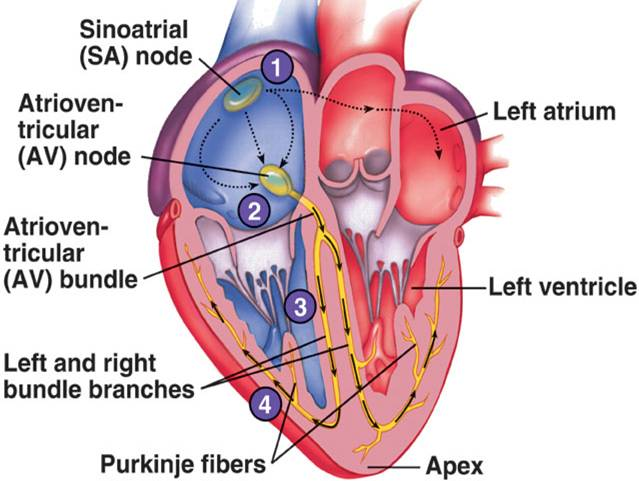
\includegraphics[width=0.9\textwidth]{bilder/b_electrical_heart}
     \caption{http://www.austincc.edu/rfofi/NursingRvw/PhysText/Cardiac.html}.
     \label{b_electrical_heart.png}
\end{figure}


%%which came first, the clot or the heart attack?


%%KILDE: file:///Users/BassE/Downloads/9781461461432-c1.pdf









